% ----------------------------------------------------------------------
\renewcommand{\CurrentProgressBarIs}{\ThreeOfFive}
% ----------------------------------------------------------------------
\begingroup
% \setbeamercolor{normal text}{bg=black}
\setbeamercolor{background canvas}{bg=mLightBrown!10}
\begin{frame}[t,plain]{3. Biomedical word sense disambiguation (BioWSD)}
\end{frame}
\endgroup
% ----------------------------------------------------------------------
\begingroup
\setbeamercolor{background canvas}{bg=mLightBrown!10}
\begin{frame}[t]{3. Biomedical word sense disambiguation (BioWSD)}

\centering
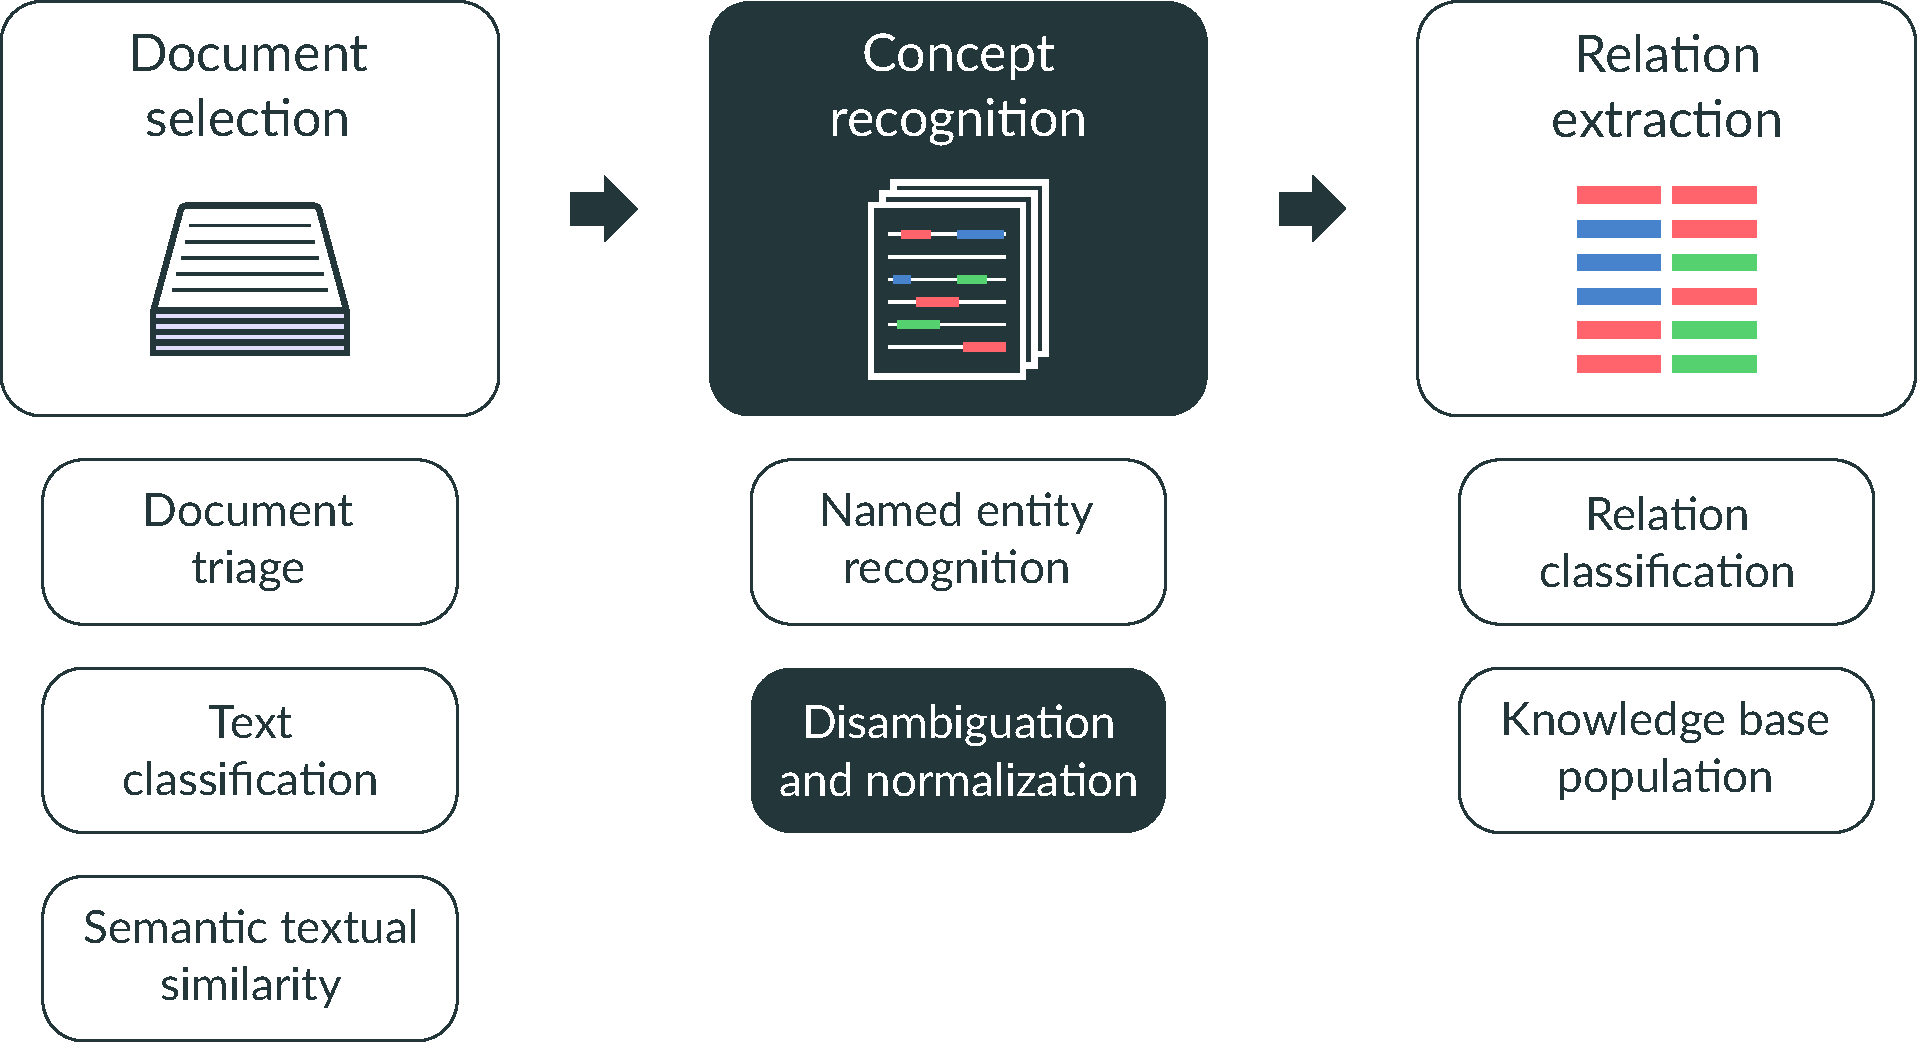
\includegraphics[width=0.80\textwidth]{img/biomedical-information-extraction/v3/006.pdf}%

\end{frame}
\endgroup
% ----------------------------------------------------------------------
\begin{frame}[t]{BioWSD: Problem and dataset}

\centering

% \vspace*{-4mm}
% \vspace*{-2mm}
% \vspace*{2mm}
% \vspace*{4mm}

% \begin{itemize}
% \item
% Assign a \alert{unique meaning} to an ambiguous term
% \end{itemize}

% Considering the expression:
\begingroup\Large%\normalsize
\textit{carcinogens in \alert{drinking} water}
% \textit{carcinogens in \alert{drinking} water}
% \textit{carcinogens in \alert{drinking} water} $\rightarrow$ \texttt{['carcinogens', 'in', \alert{'drinking'}, 'water']}
\endgroup

\vspace*{4mm}

\begingroup%
\renewcommand*{\arraystretch}{1.2}%
\setlength{\tabcolsep}{12pt}%
\begin{tabular}{l@{\hskip8pt}lll}
                   & \textbf{Concept}  & \textbf{CUI} & \textbf{MeSH}\\[4pt]
{\footnotesize\cxmark} & Alcohol drinking  & C0001948     & D000428\\
{\footnotesize\ccmark} & Water consumption & C0684271     & D004326\\
\end{tabular}
\endgroup

\vspace*{5mm}

\flushleft\small
\textbf{MSH WSD dataset}%
\vspace{-0.6\topsep}%
\begin{itemize}%
\setlength{\itemsep}{-4.0pt plus 2.0pt minus 1.0pt}%
\item
203 ambiguous terms
\item
37\,888 ambiguity cases
\end{itemize}

% \bigskip
\medskip
% \smallskip

\fontsize{5pt}{6pt}\selectfont
\begin{tabular}{@{}l@{\hskip2pt}l}
Source: & Antonio Jimeno-Yepes, Bridget T. McInnes, and Alan R. Aronson (June 2011).\\
& \textit{Exploiting MeSH indexing in MEDLINE to generate a data set for word sense disambiguation}. BMC Bioinformatics.\\
& \url{https://lhncbc.nlm.nih.gov/ii/areas/WSD/collaboration.html}
\end{tabular}

\end{frame}
% ----------------------------------------------------------------------
\begin{frame}[t]{BioWSD: Approaches}

\vspace*{6mm}

\begingroup
\begin{tabular}{l}
{\large Knowledge-based}\\
\midrule
Word embeddings $\cdot$ CUI textual definitions $\cdot$ Cosine similarity\\
\end{tabular}
\endgroup

\bigskip
\bigskip
\bigskip

\begingroup
\begin{tabular}{l}
{\large Supervised}\\
\midrule
Bag-of-words $\cdot$ Word embeddings $\cdot$ Machine learning classifiers\\
\end{tabular}
\endgroup

\end{frame}
% ----------------------------------------------------------------------
\begin{frame}[t]{BioWSD: Knowledge-based method}

% \centering

\vspace*{-3mm}
% \vspace*{4mm}

\newcommand{\mybullet}{\raisebox{0.6pt}{$\bullet$}}

\begin{columns}[t,totalwidth=\textwidth]

\begin{column}{0.40\textwidth}

% \centering

\begingroup\normalsize%
\textit{carcinogens in \alert{drinking} water}\\[12pt]
\footnotesize%
\setlength{\tabcolsep}{1.5pt}%
\begin{tabular}{@{}ll}
\mybullet\ \ Ambiguous term: & \textit{drinking}\\
\mybullet\ \ Context t: & \textit{carcinogens in water}
\end{tabular}
%%%%% % Context:
%%%%% Context $\mathbf{t}$:
%%%%% % In fact \mathbf{} is using Lato font type.
%%%%% % Apparently, Libertinus Math has no bold font face.
%%%%% % Context $\textbf{t}$:\\
%%%%% % Context $\mathbf{t}$:\\
%%%%% \textit{carcinogens in water}
\endgroup

\vspace*{10mm}

\begingroup\footnotesize%
\renewcommand*{\arraystretch}{0.95}%
\setlength{\tabcolsep}{12pt}%
\begin{tabular}{@{}l@{\hskip4pt}l@{\hskip8pt}l}
& \textbf{Concept} & \textbf{CUI}\\%[4pt]
\cxmark & {\color{Firebrick3}Alcohol drinking} & {\color{Firebrick3}C0001948}\\
\ccmark & {\color{mLightGreen}Water consumption} & {\color{mLightGreen}C0684271}\\
\end{tabular}
\endgroup

\vspace*{8mm}

\end{column}

\begin{column}{0.60\textwidth}

\RaggedLeft
\vspace*{2mm}
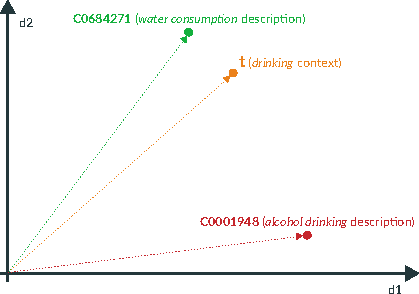
\includegraphics[width=0.90\textwidth]{img/wsd-example/v5/001.pdf}%

\end{column}

\end{columns}

\end{frame}
% ----------------------------------------------------------------------
\begin{frame}[t]{BioWSD: Knowledge-based method}

\vspace*{-3mm}
\small
\textbf{Word embeddings weighting}

% \vspace*{4mm}

\footnotesize
\vspace*{-0.4\topsep}
\begin{itemize}
\setlength{\itemsep}{-2.0pt}
% \setlength{\itemsep}{20.0pt plus 2.0pt minus 1.0pt}
\item
Term frequency--inverse document frequency (TF--IDF)
\item
Word distance decay (and IDF)
\end{itemize}

\vspace*{6mm}
\centering
\scriptsize

% \begingroup%\large
% \textit{carcinogens in \alert{drinking} water} $\rightarrow$ \texttt{['carcinogens', 'in', \alert{'drinking'}, 'water']}
% \endgroup

\begingroup%\large
\small\textit{carcinogens in \alert{drinking} water}
\endgroup

\vspace*{3mm}

\begin{center}
\renewcommand*{\arraystretch}{0.9}%
\begin{tabular}{llF{30mm}F{30mm}F{30mm}}
% \toprule
& & \texttt{'carcinogens'} & \texttt{'in'} & \texttt{'water'}\\
% \midrule
\cmidrule{2-5}
& $d$ (distance) & \texttt{2} & \texttt{1} & \texttt{1}\\
% \midrule
\cmidrule{2-5}
$\mathrm{f}(d)$ & $1$                       & \texttt{1.0000} & \texttt{1.0000} & \texttt{1.0000}\\
                & $1/d$                     & \texttt{0.5000} & \texttt{1.0000} & \texttt{1.0000}\\
                & $\exp{\left(-d\right)}$   & \texttt{0.1353} & \texttt{0.3679} & \texttt{0.3679}\\
                & $1/\ln{\left(1+d\right)}$ & \texttt{0.9102} & \texttt{1.4427} & \texttt{1.4427}\\
% \bottomrule
\end{tabular}
\end{center}

\end{frame}
% ----------------------------------------------------------------------
\begin{frame}[t]{BioWSD: Knowledge-based method}

\vspace*{-2mm}
% \vspace*{6mm}

\begingroup\footnotesize\renewcommand*{\arraystretch}{0.9}%
\begin{tabular}{l}
% {\small Knowledge-based}\\
% \midrule
Word embeddings $\cdot$ CUI textual definitions $\cdot$ Cosine similarity\\
\qquad\alert{Word embeddings averaging functions}
\end{tabular}
\endgroup

\vspace*{5mm}

\begin{columns}[t,totalwidth=\textwidth]

\begin{column}{0.40\textwidth}
\large%
\vspace*{-40mm}
% \centering
\begin{align*}
\mathrm{score}({\color{DarkOrchid1}\mathrm{CUI}}) = \mathrm{CS}(\alert{\mathbf{t}}, {\color{DarkOrchid1}\mathbf{CUI}})
\end{align*}
\end{column}

\begin{column}{0.60\textwidth}
% \RaggedLeft
\centering
% \vspace*{2mm}
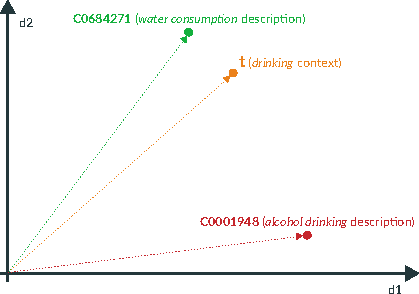
\includegraphics[width=0.84\textwidth]{img/wsd-example/v5/001.pdf}%
\end{column}

\end{columns}

\end{frame}
% ----------------------------------------------------------------------
\begin{frame}[t]{BioWSD: Knowledge-based method extended}

\vspace*{-2mm}
% \vspace*{6mm}

\begingroup\footnotesize\renewcommand*{\arraystretch}{0.9}%
\begin{tabular}{l}
% {\large Knowledge-based}\\
% \midrule
Word embeddings $\cdot$ CUI textual definitions $\cdot$ Cosine similarity\\
\qquad Word embeddings averaging functions\\
\qquad\alert{CUI--CUI association values (NPMI)}
\end{tabular}
\endgroup

\vspace*{0.475mm}

\begin{columns}[t,totalwidth=\textwidth]

\begin{column}{0.40\textwidth}
\small % 10pt
% \footnotesize % 9pt
% \scriptsize % 8pt
% \fontsize{7.0pt}{8.4pt}\selectfont
% \tiny % 6pt
% \fontsize{5pt}{6pt}\selectfont
% \fontsize{4pt}{4.8pt}\selectfont
\vspace*{-40mm}
% \centering
\begin{align*}
& \mathrm{score}({\color{DarkOrchid1}\mathrm{CUI}}) =\\[6pt]
& \frac{1}{N} \sum\limits_{j}{} \mathrm{NPMI}({\color{DarkOrchid1}\mathrm{CUI}}, \mathrm{CUI}_j) \cdot \mathrm{CS}(\alert{\mathbf{t}}, \mathbf{CUI}_j)\\
\end{align*}
\end{column}

\begin{column}{0.60\textwidth}
% \RaggedLeft
\centering
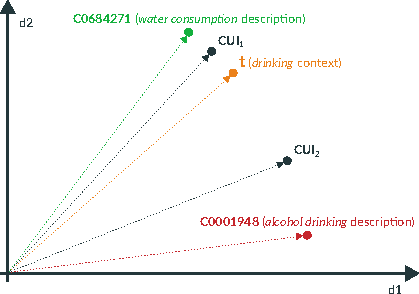
\includegraphics[width=0.84\textwidth]{img/wsd-example/v5/002.pdf}%
\end{column}

\end{columns}

\end{frame}
% ----------------------------------------------------------------------
\begin{frame}[t]{BioWSD: Knowledge-based method extended}

\textbf{CUI--CUI association values}

\begin{itemize}

\item
MeSH (CUI) co-occurrences in MEDLINE citations

% \pause
% \item
% MeSH--CUI mapping

\item
Normalized pointwise mutual information (NPMI)

\end{itemize}

\bigskip

\begin{center}\small
\begin{tabular}{|F{18mm}|F{18mm}F{18mm}F{1cm}F{18mm}@{}m{0pt}@{}}
\cline{2-5}
\multicolumn{1}{c|}{NPMI} & \multicolumn{1}{c|}{C0000039} & \multicolumn{1}{c|}{C0000052} & \multicolumn{1}{c|}{\ldots} & \multicolumn{1}{c|}{C4076759} &\\
\cline{1-5}
C0000039 & \texttt{1.00} & \texttt{0.23} & \ldots & \texttt{0.37} &\\
\cline{1-1}
C0000052 & \texttt{0.23} & \texttt{1.00} & \ldots & \texttt{0.68} &\\
\cline{1-1}
\ldots & \ldots & \ldots & \ldots & \ldots &\\
\cline{1-1}
C4076759 & \texttt{0.37} & \texttt{0.68} & \ldots & \texttt{1.00} &\\
\cline{1-1}
\end{tabular}
\end{center}

\end{frame}
% ----------------------------------------------------------------------
\begin{frame}[t]{BioWSD: Knowledge-based results (accuracy)}

\centering
% \footnotesize
\scriptsize

% \vspace*{2mm}
% \bigskip

% \renewcommand*{\arraystretch}{0.8}

\begin{tabular}{D{22.0mm}G{6.0mm}G{14.0mm}G{14.0mm}G{14.0mm}G{14.0mm}G{14.0mm}}
% \toprule
\textbf{CUI--CUI} & \multicolumn{1}{l}{\textbf{WE}} & \multicolumn{5}{l}{\textbf{Weighting scheme}}\\

\textbf{associations} & \multicolumn{1}{l}{Size} & \multicolumn{1}{r}{Term frequency} & \multicolumn{1}{r}{No decay} & \multicolumn{1}{r}{Fractional} & \multicolumn{1}{r}{Exponential} & \multicolumn{1}{r}{Logarithmic}\\

\midrule

CS & 100 & 0.8321 & 0.8341 & 0.8502 & 0.8278 & 0.8468\\[2pt]
   & 300 & 0.8337 & 0.8365 & \textbf{0.8533} & 0.8276 & 0.8501\\

\midrule

NPMI \geq\ 0.8 & 100 & 0.8314 & 0.8334 & 0.8493 & 0.8264 & 0.8461\\[2pt]
               & 300 & 0.8332 & 0.8357 & \textbf{0.8518} & 0.8264 & 0.8491\\

\midrule

NPMI \geq\ 0.5 & 100 & 0.8197 & 0.8236 & 0.8376 & 0.8150 & 0.8343\\[2pt]
               & 300 & 0.8209 & 0.8245 & \textbf{0.8396} & 0.8168 & 0.8352\\

\midrule

NPMI \geq\ 0.3 & 100 & 0.8600 & 0.8635 & \underline{\textbf{0.8744}} & 0.8459 & 0.8730\\[2pt]
               & 300 & 0.8582 & 0.8611 & 0.8736 & 0.8478 & 0.8719\\

% \bottomrule

\end{tabular}

\vspace*{8mm}
\RaggedRight
* 5-fold cross-validation

\end{frame}
% ----------------------------------------------------------------------
\begin{frame}[t]{BioWSD: Supervised machine learning results (accuracy)}

\centering
% \footnotesize
\scriptsize

% \vspace*{2mm}
% \bigskip
% \medskip

\renewcommand*{\arraystretch}{0.9}

\newcommand{\z}{\hphantom{0}}
\begin{tabular}{D{13.3mm}D{5.0mm}D{11.0mm}G{12.2mm}G{12.2mm}G{12.2mm}G{12.2mm}G{12.2mm}}
% \toprule

\textbf{BoW} & \multicolumn{2}{l}{\textbf{WE}} & \multicolumn{5}{l}{\textbf{Classifier}}\\
Features & Size & Window & DT & kNN & LR & MLP & SVM\\

\midrule

U   & \z\z- & \z- & 0.9067 & 0.9324 & 0.9205 & 0.9401 & 0.9511\\
B   & \z\z- & \z- & 0.8335 & 0.8850 & 0.8704 & 0.9224 & 0.9253\\
U+B & \z\z- & \z- & 0.9019 & 0.9354 & 0.9101 & 0.9445 & \textbf{0.9552}\\

\midrule

- & 100 & \z5 & 0.9219 & 0.9452 & 0.9500 & 0.9503 & 0.9449\\
- &     &  20 & 0.9185 & 0.9452 & 0.9495 & 0.9498 & 0.9452\\[2pt]
- & 300 & \z5 & 0.9186 & 0.9449 & 0.9505 & 0.9503 & 0.9452\\
- &     &  20 & 0.9186 & 0.9444 & 0.9508 & \textbf{0.9514} & 0.9446\\

\midrule

U & 100 & \z5 & 0.9244 & 0.9464 & 0.9515 & \underline{\textbf{0.9557}} & 0.9490\\
  &     &  20 & 0.9215 & 0.9468 & 0.9514 & 0.9556 & 0.9486\\[2pt]
  & 300 & \z5 & 0.9218 & 0.9475 & 0.9519 & 0.9544 & 0.9499\\
  &     &  20 & 0.9194 & 0.9473 & 0.9524 & 0.9550 & 0.9496\\

% \bottomrule

\end{tabular}

\vspace*{4mm}
\RaggedRight
* 5-fold cross-validation

\end{frame}
% ----------------------------------------------------------------------
\begin{frame}[t]{BioWSD: Comparison with other works (accuracy)}

\centering
% \footnotesize % 9pt
% \scriptsize % 8pt
\fontsize{7.0pt}{8.4pt}\selectfont
% \tiny % 6pt
% \fontsize{5pt}{6pt}\selectfont
% \fontsize{4pt}{4.8pt}\selectfont

% \vspace*{2mm}
% \bigskip
% \medskip
% \smallskip

\renewcommand*{\arraystretch}{1.1}

\newcommand{\etal}{\textit{et al.}}
\newcommand{\z}{\hphantom{0}}
\begin{tabular}{D{48mm}D{43mm}G{12mm}G{20mm}}

% \toprule

Work & Approach & Supervised & Knowledge-based\\

\midrule

Zhang, Biś, Liu, and He (2019)             & Long short-term memory networks & 0.9600 & -\\
Pesaranghader, Matwin \etal\ (2019)        & Long short-term memory networks & 0.9682 & 0.9267\\
Duque, Stevenson \etal\ (2018)             & Co-occurrence graph & - & 0.7152\\
\alert{Ours (Antunes and Matos, 2017)}     & \alert{Word embeddings, cosine similarity} & \alert{0.9557} & \alert{0.8744}\\
Jimeno-Yepes (2017)                        & Support vector machine & 0.9597 & -\\
Sabbir, Jimeno-Yepes, and Kavuluru (2016)  & Word embeddings, k-nearest neighbors & - & 0.9434\\
Tulkens, Šuster, and Daelemans (2016)      & Word embeddings, cosine similarity & - & 0.84\z\z\\
Jimeno-Yepes and Berlanga (2015)           & Word--concept statistical model & 0.930\z & 0.891\z\\
McInnes and Stevenson (2014)               & Semantic similarity measures & 0.97\z\z & 0.78\z\z\\
McInnes and Pedersen (2013)                & Semantic similarity measures & - & 0.75\z\z\\
Garla and Brandt (2013)                    & Semantic similarity measures & - & 0.8071\\
Jimeno-Yepes, McInnes, and Aronson (2011)  & Naive Bayes classifier & 0.9386 & 0.8383\\

% \bottomrule

\end{tabular}

\end{frame}
% ----------------------------------------------------------------------
